\documentclass[11pt]{article}
\usepackage[usenames,dvipsnames]{xcolor}
\usepackage{soul}
\usepackage{graphicx}
\usepackage{lineno}
%\linenumbers

\usepackage{hyperref}
\usepackage{booktabs}

%\usepackage{amssymb}
\usepackage{xspace}
\usepackage{graphicx}
%\usepackage{todonotes}
\usepackage{ifthen}

\usepackage{geometry}

\topmargin 0.0cm
\oddsidemargin 0.2cm
\textwidth 16cm 
\textheight 21cm
\footskip 1.0cm

% Remove the "Contents" label from the Table of Contents
\makeatletter
\renewcommand\tableofcontents{%
    \@starttoc{toc}%
}
\makeatother

\begin{document}

\newif\ifone
\newif\iftwo
\newif\ifthree
\newif\ifhlt

\onetrue % Response to referee 1
\onefalse
\twotrue % response to referee 2
\twofalse
\threetrue % response to referee 3
%\threefalse
%\hlttrue  % Highlighting page number checks
\hltfalse

\ifone
\newcommand{\one}[2]{\textbf{\textcolor{blue}{1: #1}}\\ \linebreak {#2}\\\noindent\rule{\textwidth}{1pt}\bigskip}
\else
\newcommand{\one}[2]{}
\fi

\iftwo
\newcommand{\two}[2]{\textbf{\textcolor{teal}{2: #1}}\\ \linebreak {#2}\\\noindent\rule{\textwidth}{1pt}\bigskip}
\else
\newcommand{\two}[2]{}
\fi

\ifthree
\newcommand{\three}[2]{\textbf{\textcolor{Maroon}{3: #1}}\\ \linebreak {#2}\\\noindent\rule{\textwidth}{1pt}\bigskip}
\else
\newcommand{\three}[2]{}
\fi

\ifhlt
\newcommand{\hlt}[1]{\hl{#1}}
\else
\newcommand{\hlt}[1]{{#1}}
\fi



\begin{center}
\textbf{\Large{Response to Referees}}\\
\smallskip
\today
\end{center} 
\medskip

%\title{Response to Referees}
%\maketitle
%\vspace{-5mm}

We would first like to convey to the referees the same sentiment that we have expressed to the editor: we are sincerely grateful that you are willing to still consider this manuscript after such an extraordinarily long delay.  This past year has been challenging in many ways, and we are deeply appreciative of your openness to review this resubmission. 

The comments from all three referees were very constructive.  Many required significant thought and effort to respond to, and we feel that the paper has improved in the process.  We do hope that the referees will agree, and look forward to learning what you think of the updated manuscript.

Our point-by-point responses are presented below. In this document we have grouped the responses by topic and area of the manuscript, so that referees can see responses to similar concerns in context.   We have color-coded each referee's comments, matching the colors used in the changetext version of the manuscript, as follows:

\begin{itemize}
\item \textbf{\textcolor{blue}{Items from Referee \#1 in blue.}}
\item \textbf{\textcolor{teal}{Items from Referee \#2 in teal.}}
\item \textbf{\textcolor{Maroon}{Items from Referee \#3 in maroon.}}
\end{itemize}

After each item we provide our response in black text.  Page references and line numbers refer to the lines in the ``changetext'' version of the manuscript.

We have provided our response to editorial suggestions in a separate cover letter, but the referees should note that we have re-worded the first paragraph to follow the guidelines provided by the editor, and we have removed some references as we added new ones, in order to keep to the guidelines.  All changes made in response to editorial comments are  \textbf{\textcolor{violet}{in purple text}} in the changetext document.

The sections of this response are as follows: \\
\bigskip

\tableofcontents

\clearpage

\section{Overall Significance}

\one{The authors have discovered a unique and interesting gravitational lens system whose predictions of a future event, if correct, could help put constraints on some of the cosmological parameters. The manuscript, generally, reads well. The reasons to publish this in Nature Astronomy are not obvious though. The authors make a good case that the transient source is a lensed SN of type 1a and since this is not still confirmed, one cannot rule out the possibility that it may be of a different type. In any case, there have been other lensed SN Ia detections (e.g. Quimby et al. 2014, Goobar et al. 2017) although not with long time delays. Furthermore, had this been the analysis of their model predicted event, it would be a first such analysis, of high significance and relevance to the wider community and thus, suitable for Nature Astronomy.\\ 
In light of these statements, could the authors justify the suitability of their choice of journal in a few sentences ?}
{Our perspective is that articles published in Nature Astronomy should be broad and significant: of interest to a broad range of astronomers, and presenting significant new discoveries or theoretical models.
\begin{itemize}
\item On breadth, this touches on a wide range of subjects astronomy—gravitational lensing, transient surveys, SN science, cosmology, and galaxy evolution.  The breadth is also highlighted by its relevance for the Rubin Observatory and Roman Space Telescope. 
\item  As for the significance, we believe that this discovery will be important in supporting the role of cluster-scale lensing for future SN time delay cosmography programs.  When review articles are written in a decade, we expect this transient will be listed alongside SN Refsdal as a trailblazer for the use of cluster-lensed SNe in cosmology.
\end{itemize}
As you will see in further responses below, even though SN Refsdal was lensed by a galaxy cluster, since its discovery in 2015 the vast majority of the literature on lensed SN has focused on the prospects for building cosmological samples from galaxy-lensed SNIa like SN 2016geu. Furthermore, SN Refsdal required dozens of HST orbits over several years of monitoring and follow-up. With SN Requiem we are demonstrating that cosmologically useful time delays can be measured with minimal observational cost using cluster-lensed SNe. This event is ready and waiting for the final time-delay measurements with just two epochs of imaging. The long time baseline virtually ensures that this event will deliver a time delay measurement with sub-percent precision, making this class of lensed SN a very low-cost but high-value target population.}

\one{The authors make an important point about the utility of cluster scale lenses with long time delays for cosmology given that most lenses will be at galaxy scales with short time delays and affected by microlensing. Why do the authors think that the VRO survey won't find cluster scale lensed SNe ? Assuming that they can be found, the projected constraints in Fig. 3 may then be biased corresponding to the VRO sample, at least. Similar revision for RST may be required too.
}{This is a very valid point, and we've attempted to clarify this in the text on \hlt{page 7 (blue text, line 134-135).} In brief, the VRO and Roman lensed SN samples will indeed include cluster-lensed SNe, but almost all previous analyses of these surveys have been limited to galaxy-scale lenses.\\
For brevity, we did not expand on the literature context in the text, but we will here. :\\
- Oguri \& Marshall 2010 did not consider clusters. They were limited only to elliptical galaxy lenses (which they assessed would make up $>80\%$ of all lensed transients in modern wide-field surveys.)\\
- Goldstein \& Nugent 2017, Goldstein et al. 2019 and Wojtak et al. 2019 were also all limited to elliptical galaxy lenses.\\
- Pierel et al. 2021 analyzed the Roman Space Telescope, considering only galaxy-scale lenses.\\
- Petrushevska et al. 2018 and Petrushevska 2020 have addressed cluster-lensed SNe, but they have explicitly limited those analyses to time delays $<5$ years, because of the JWST lifetime.  Note that we have added these references in the ``Future Discoveries" discussion \hlt{in the Supplemental Note, p 42-43)}.}

\one{On a related point, it is unclear what kind of lenses were used for the simulations of VRO and RST survey samples and what properties are considered when the authors simulated ``AT 2016tbd-like" ? The text suggests something regarding the ratio of the source redshift to lens redshift but what about other parameters such as the lens mass scales, redshift range, time delays ? How do they compare with the J0138 lens?}{The simulated ``AT 2016tbd-like" sample is constructed to mimic the time delay and redshift properties of the discovered object. That is, we have assumed a redshift ratio that matches the observed redshift ratio of SN AT 2016tbd, and we have assumed that the time delay can be measured to $<1\%$ precision, as would be the case for other cluster-scale lenses with decade-long lensing time delays.  This has been clarified in the text \hlt{(page 7, blue text, lines 148-149)}}

 
\one{What is going to be the significance of the analysis of this system in 2037, assuming many more lensed SNe are likely to be found by planned and future surveys? Note that it is unlikely we will have only about 5 systems with long time delays in the next 17 years. A sentence on this point needs to be added.}{
We do not expect that this system alone will stand out as a singularly important system in 2037, in the same way that one of the Type Ia SNe like SN 1991T or SN 1991bg was not particularly important in and of itself after a decade. As with those seminal Type Ia discoveries, the value of this system will be that it provides a benchmark for a class of objects that can collectively be important for lensed time delay cosmology. A sentence reflecting this has been added \hlt{(page 7, lines 131-132)}}

\two{On a more general note, it would be surprising to most if 20 years from now, with the slew of ground and space-based cosmology surveys in the pipeline, current day precision estimates of the Hubble constant and the Dark Energy equation of state parameters are a relevant point of comparison. Thus, it is hard to get excited about potentially(!) getting a precise time-delay estimate 17 years from now.}{

This is fair enough.  However, you could also ask how many in the cosmological community would have predicted in the year 2000 that a tension in the measurement of $H_0$ would be a hot topic in 2020? 

We don't really know what is coming 10 or 20 years from now, but the strength of the dark energy enterprise is in the many complementary methods we have available.      Anticipating this precise time delay in 17 years should motivate us to continue building the tools to make cluster-lensed SNe a more fully developed part of that cosmology toolkit.
} 


\section{Supernova Classification}

\one{Fig. 2 Right panel: There's no comment about the fact that the best-model-predicted-unlensed magnitudes of images 1-3 are above the curve showing the evolution.}{
\textit{Note that this figure has been reconstructed, so the panel referenced is now panel (c)}\\
A number of effects could account for this, though we would caution readers not to over-interpret the limited data (granting that we ourselves are doing everything we can to squeeze reasonable inferences out of these few data points).    We have added a brief comment in the text addressing this (page 5, blue text, lines 89-93). \\
  For the interested referee, we elaborate:\\
- The well-known mass sheet degeneracy (MSD) is one plausible explanation, in which an intervening mass sheet between the observer and the lens can systematically shift the absolute magnifications of all background sources, without altering their relative magnifications, or the apparent positions of the multiple images (Falco, Gorenstein \& Shapiro 1985).   Note that the MSD would also not impact the time delay predictions or observations.  More general related degeneracies can have similar systematic effects (Schneider \& Sluse 2014).   Impacts of these degeneracies can be mitigated by including many multiply imaged systems at different redshifts as input constraints for the lens models, and including spatially resolved kinematics of the lensing system (e.g. Birrer et al. 2016, Shajib et al. 2019).\\
- If the points had landed below the curve in the right side of Fig 2, then this source would have looked more consistent with the CC SN population.  Invoking the MSD or a similar degeneracy might then have been an important consideration in evaluating the classification of the source.  However, since the points fall above the line (brighter than expected), this makes the source even less likely to be a CC SN (one would need to invoke an even stronger mass sheet effect to bring those points into the CC region of the diagram. \\
- The key takeaway we would like readers to get from that panel of the figure is that the three points follow the trend that would be expected for a Type Ia SN evolving over time.  They are consistent with the curve, and the offset could reasonably be explained by a well-known lensing effect.}

\bigskip
\textit{Several comments from referee 2 raise concerns related to the classification reported in the Table S6 and Figure S2. \hlt{(NOTE: Table S6 is now Table 7 on p.23.   Fig. S2 is now Fig. 6 on p.24)}}
\medskip

\two{Issue \#1: Classification\\
It is of course painful that the late discovery of the 2016 transient, a presumed supernova explosion, prohibits spectroscopic identification and photometric follow-up which would have allowed a proper classification of the transient, as well as establishing accurate times for a later time-delay measurement.\\\\
The authors have tried very hard to overcome these shortcomings by using both the properties of the presumed host galaxy at z=1.95 as well as the HST NIR imaging in two bands from 2016, when three images of the transient were detected. However, while certainly plausible, I find that the authors fail to present a clear case for the ``90\%" confidence of this being a Type Ia supernova. Figure 2 in the main journal article is what the authors have chosen to demonstrate this. I find this figure quite hard to read and interpret I can agree that it shows that a SNIa classification is acceptable, while I cannot really tell if other classifications are significantly worse. This becomes even more problematic while looking at Fig. S2, where I find it quite unlikely that the authors can make claim that the dotted line (SNII) is a worse statistical fit than the solid line (SNIa).}{
The referees have identified a clear failing in the presentation of this photometric SN classification.  As previously constructed, Fig 6 (formerly S2) was visually misleading, because the light curve models shown were the maximum-likelihood fits.  As such, they were only showing a goodness-of-fit, not a true posterior probability.    As previously noted in the text of the supplemental materials: \\\\
``This figure shows that the limited photometric data can be reasonably well fit by at least one model from any of these three sub-classes. However, the range of model parameters that allow such a fit to the data is much more limited for the heterogeneous CCSN types than for the Type Ia class."\\\\
When computing a full posterior probability, the STARDUST2 algorithm computes the likelihood over a wide range of CC SN models (light curve templates) and model parameters (time of peak, luminosity, host galaxy dust extinction).   The total Type Ia classification likelihood is also computed by marginalizing over a wide range of light curve parameters for the SALT2 model (t0, x0, x1, c).   Therefore the previous Figure S2 was not very informative, because it only showed that any of these SN sub-classes could provide a good fit to the data with at least 1 set of parameters.\\\\
We have now provided a new figure 6 that shows a representative set of light curves and F105W-F160W color curves from the STARDUST2/sncosmo nested sampling chains.   This shows that although there are a few examples of Type Ib/c or Type II models that can fit these data with a low $\chi^2$, there is a much greater density of Type Ia instances that do as well or better.   The net effect is that the Type Ia likelihood distribution has a broad plateau of high likelihood across parameter space, while the CC distributions have a few spikes with a much wider region of low likelihood.  Multiplying each of these likelihood landscapes by the host galaxy priors serves to further enhance the Type Ia posterior probability relative to the collective Core Collapse posterior.  
}

\two{Moreover, when it comes to all the non-Ia supernovae alternatives, the authors are no longer dealing with ``standard candles". Thus, while the SED templates used produce some sort of generic behavior for the bulk of core-collapse supernovae subtypes, individual light curves observed in the local universe show a great deal of diversity within the same sub-type classification, rendering a classification based on such limited data and strong assumptions very doubtful.}{
It is certainly true that we should not take the limited set of CC SN SED templates as fully representative of the CC SN subtypes.  This is exactly why we begin our classification by comparing the photometry against a smoothed representation of the entire population for each subtype, in color-magnitude space (Fig 2a, and again in Fig 4 in the Methods).   In these figures, the gaps in the SN template library are smoothed over by random sampling and removal of the time dimension.  We can already see that the three observed data points are much more consistent with the red ``Type Ia" cloud than either of the CC SN clouds.   Combining this ``birds eye view" with the more granular light-curve and color-curve view in the revised Figure 6, we believe that we've now given solid visual support for the quantitative classification probabilities reported in the text. \\\\
We do acknowledge that this methodology is imperfect, especially when applied at high redshift where the SN populations may have systematic differences due to demographic evolution.    However, this approach is not dissimilar to the classification used for other SN at similar redshift and with similarly limited photometric information.   For example, see: \\
\url{https://ui.adsabs.harvard.edu/abs/2018ApJ...866...65R/abstract}\\
\url{https://ui.adsabs.harvard.edu/abs/2018MNRAS.479.3563F/abstract}\\
\url{https://ui.adsabs.harvard.edu/abs/2013ApJ...768..166J/abstract}
}

\two{Furthermore, the identification makes use of the LENSTOOL estimates of the time-delays to spread the measured photometry in time. Examination of table S7 with the 5 lensing models shows dramatic differences in establishing the relative age of the SN images at the time of observations.}{
It is very true, as Referee \#2 points out, that all of this photometric classification is strongly conditional on both the presumptions of SN population correlations with host galaxy properties, and on the adoption of magnification corrections from the lens model.  Please note, however, that the classification of this source as a likely Type Ia SN does not rely strongly on the lens-model-predicted time delays.  The classification information summarized in Figure 2 reflects the classification result of p(Ia)=0.95 that appears as row (c) in Table 7.   This was made without including any time delay correction.   As shown in Figure 2b, the color-magnitude data alone is suggestive of a time delay of ~100 days between image 2 and images 1+3, if this is a Type Ia SN.  We feel that the overall Type Ia classification inference is strengthened by the fact that the lens model independently (and in a blinded analysis) predicted roughly that same time delay.\\ \\
When we do include the lens model time delay to put the three points together as a single light curve for classification, we find an almost identical classification probability:  p(Ia)=0.94, reported in row (d) on Table 7.   This reinforces the fact that the lens model time delay is not introducing new information that is essential to the classification. \\\\
 If any of these priors are changed (by future observations or new lens modeling) then the classification should be updated accordingly, as a good Bayesian does.   We have attempted to include appropriate caveats throughout the text, though most of these are in the supplemental material.   Although we prefer to be quantitative when presenting results, we acknowledge that the subtleties of classification are elided by the headline statement in the abstract of ``>90\% probabibilty".    To make the reader more immediately aware of the limitations of the classification evidence, we have changed this to a ``likely" classification, which is a little squishy, but certainly encompasses the range of 60-95\% classification probabilities presented in Table 7.     When we present the classification in the main text we have also added a statement to point out that we are proceeding with the assumption that this object is a Type Ia SN, but if future observations show it to be a CC SN, much of the same analysis can be repeated, simply using a different light curve model  \hlt{(page 6, line 114)}.   As long as the ages of the first three SN images  can be constrained to within $\pm$300 days (not a high bar), the time delay measurements will have better than 4\% precision and be subdominant in the error budget of any cosmological inference.}

\two{While the nature of the host galaxy is suggestive of a SNIa host in the local universe, however, it is hard to quantify the applicability of this inference at redshift 2.}{
It is true that there are not enough SN detections at z$\sim$2 for us to rely only on a purely empirical approach to correlating SN class with host galaxy properties.  However, for this host we have not only the observables (luminosity, color) but we also know something about the physical properties of the galaxy (mass and star formation rate).   We can therefore use a correlation to the SN population that is strongly physically motivated: the progenitors of CC SNe are more massive than Type Ia SN progenitors, so when a galaxy has an older stellar population we should expect that it will preferentially host Type Ia SNe over CC SNe.  \\\\
In Table 7 we have presented both of these possible host-based classifications.   Row (a) shows that we infer p(Ia)=0.75 when considering the host galaxy's bulk observed properties ($M_K$ and $B-K$).   This is the inference that should be treated as most suspicious when translated to z$\sim$2.    Row (b), however, uses instead the inferred mass and star formation rate of the host galaxy, which gives us the more solid footing of a physically-motivated association to SN class. 
\\\\
You may be concerned that at high redshift we should even be suspicious of the correlation of stellar population properties with SN rates and subtypes.   To address this concern, we would refer the reader to Rubin, Hayden et al 2018 and  Meyers et al 2012, two studies from the Supernova Cosmology Project that examined this question in some detail, for SN host galaxies that are quite similar to the one presented here.   Those authors consistently found that the host galaxy physical properties remain a reliable indicator for SN Ia classification even at z>1.5. 
\\\\
In our analysis we adopt the physically-motivated host galaxy classification (row b of Table 7) as the prior for all subsequent classification probabilities. 
\\\\
\url{https://ui.adsabs.harvard.edu/abs/2012ApJ...750....1M}\\
\url{https://ui.adsabs.harvard.edu/abs/2018ApJ...866...65R}
}

\one{ For the color-mag calculation of the host galaxy, which image was considered and what was the magnification factor used?}{
\textit{NOTE: this is referring to the method ``a'' in \hlt{Table 7 (formerly table S6).}}

In the text we have specified that 

``We adopt a lensing magnification correction using LENSTOOL model E to get MK. The B-K color is not affected by the foreground lens.''

We used image 2 and a flux-weighted mean magnification for the galaxy, which is now reported in the new \hlt{Table 7 on page 23}, part of the newly-added subsection on Comparison to Previous Lens Modeling. We verified that using either of the other host galaxy images instead does not impact the results. The text on \hlt{page 22, lines 311-314} has been updated to clarify this.
}

\two{There is one extra test the authors could try, to leave no stone unturned. The Spitzer observations from Oct 2016 could potentially have been sensitive to the restframe J-band second maximum for a SNIa at z=1.95. It would be interesting to see if these observations have any constraining power or not.}{

Great suggestion.  We evaluated the Oct 2016 Spitzer observations in IRAC CH1 and CH2.  The best chance for a detection or constraint would be for image 2, the brightest and the one at the earliest  phase.  At the time of the IRAC observations, the image 2 phase would be $\sim$67 days after peak brightness, and we would expect it to have AB magnitudes  26.1  in both Ch1 and Ch2.   Unfortunately, this is several magnitudes fainter than the 1-$\sigma$ noise floor of about 23 to 23.5 AB mags for those IRAC bands.  So we do not have any constraining power from those Spitzer observations. }

\subsection{Figure 2}

\one{Fig. 2 Caption: Sentence about open/closed markers and dotted/solid bars is confusing. Use simpler sentences.}{
The caption has been updated to be more clear.}

\three{Figure 2 (left) and Figure S1: The caption of Figure 2 states that the simulated SNe had their color-magnitude sampled uniformly in time. Does this mean that the authors simulated 10,000 different SNe, then sampled a random time on each SNe's light curve once? Does this method account for the limiting magnitude of the observed data, which might cause a bias toward certain regions in color-magnitude space (i.e. certain SNe might only be detectable at certain points in their light curve)?}{
Yes, the referee's understanding of the sampling method for this figure is exactly correct.  

The point regarding limiting magnitudes has been addressed with new text in the Methods section \hlt{(maroon text, page 25, lines 343-347):}

``Note that in this case there is no need to apply a cut to the simulated sample to account for detectability, because the 5$\sigma$ limiting magnitude of our HST observations is 26.5 AB mag, and after accounting for magnification of $\sim$1.5 mag (Table 5) this becomes $m_{lim}\sim28$ mag. This means that all the points shown in Fig. 4 (and therefore all simulated SN entering our classification counts) would be easily detectable in our HST imaging.''   
}

\three{The ``stellar-population-based host galaxy classification'' prior presumably accounts for the expected rates of the different SNe types, and is reflected in the top and right panels of Figure S1, but this doesn't seem to come across in Figure 2 (left). This could potentially be misleading, as a casual reader might look at the left panel of Figure 2 and think that an SN Ib/c isn't all that inconsistent with the data, but the prior effectively rules it out. Maybe some additional text in the caption, or some indication of the priors in the figure itself would be useful.}{
We have updated Figure 2 to include a new sub-panel (b) that shows the distribution of our SN simulation in color space, after applying the host galaxy priors (as was previously reflected in the Methods \hlt{Figure 6, formerly Fig. S1).}  The caption  of Fig. 2 also more clearly explains how the host galaxy stellar population properties that were used here.
}

\three{Figure 2 and Figure S1: Do the filled points represent the median magnitude of the images after the magnification correction? It's not clear why the solid vertical line (representing the magnification uncertainty) only extends below the filled points and not in both directions.}{
Yes, the filled points represent the magnification-corrected magnitudes.  We have attempted to make this more clear with labels in the figure, and words in the caption of Figure 2 and the text.    Given the limited space available in the main text, we have opted to keep the discussion of the asymmetric error bars in the Methods section \hlt{(maroon text, lines 265-268 on p.18-19; and see also the green text, lines 339-341 on p.25)}}


\section{Time Delay}

\one{An uncertainty of 1.5-2 yrs in the predicted event is still fairly large for the follow-up observations to ensure that the 4th image is observed at the right time. How practically feasible is it going to be to be able to follow-up and detect the SN right when it goes off?}{
This is indeed a concern.  We hope that future observations of the lensing cluster (e.g. with JWST) will provide more lens modeling constraints.   The significant redshift of the SN and the associated cosmological time dilation is also an advantage for a future monitoring campaign.  We have laid out the reasoning for this in a new subsection ``Future Observations" note in the supplemental material \hlt{(page 41-42)}}


\two{Issue \#2: time-delay\\\\
As already pointed out above, the classification can be questioned. Even assuming it is right, the authors go on to make unsubstantiated claims on how well the light curve parameters are measured, including the time of maximum, needed to measure time delay. }{
We will do our best to more clearly substantiate our results here.  Additionally, we are using open-source code, and publishing all of the measurements used in this analysis, so we hope that a reader who is still skeptical can proceed with their own analysis if needed.  } 


\two{First of all, they seem to set x1=0 in the SALT2 fit, without proper motivation. }{
The referee has raised a reasonable point that we did not explain the handling of the SALT2  x1 parameter in great detail.    If you allow x1 to float, there is no useful constraint on it, because it is quite degenerate with the time delay between the images, which is of course a free parameter in all the fits.    Because of this, in the fiducial analysis we opted to fix x1=0 throughout the time delay fitting process.    We have also tried fixing x1 to other values from -1 to +1, and the time delay results change by less than 5 days  for both the color curve and light curve fitting, which is well within all error bars.  We argue that it is justifiable to fix x1, since we expect that a full light curve of the fourth SN image will provide a tight constraint on x1, which can then be propagated back into the fitting of the SN images 1-3.   The text has been updated to explain this more clearly \hlt{(green text in the Methods, page 28-29, lines 401-410).}
}


\two{Then, they claim that they constrain the SALT “c” parameter to an accuracy of just 0.05 mag. This is hard to believe, as such good accuracy is among the best that has been achieved in SNIa cosmology based on far better data-sets. }{
It is certainly reasonable for Referee \#2 to be surprised by the precision of this constraint on the SALT2 ``c" parameter.   As we investigated this, we discovered that there was a book-keeping error in our analysis code which was indirectly related to this: we were using the wrong column from our photometry table (aperture flux instead of PSF fitting flux, but without additional uncertainty for the aperture correction).  Correcting this led to a revision of the overall constraint on SALT2 c.  We now report this as  $c=0.04^{+0.05}_{-0.07}$.    In spite of this slightly larger uncertainty,  the referee's concern should still apply.

There are two components that lead to this unexpectedly precise measurement:

\begin{enumerate}
\item{The photometry is uncharacteristically good, especially for the brightest image (SN image 2).  This image has an AB magnitude of 23 in F105W (Y band) and 23.8 in F160W (H band) (see Table 3).  It was observed with a full 2 HST orbits of exposure time ($\sim$1.5 hours) over those two bandpasses.  The vast majority of Type Ia SNe in the literature do not have HST photometry at all, and this may be among a very few SN to get such an investment of exposure time on a single epoch at this magnitude.    The HST WFC3-IR ETC estimates that the S/N for a point source at this magnitude and exposure time should be  S/N$\sim$200 in F105W and  S/N$\sim$125 in F160W.   Our photometry measured S/N = 173 for F105W and S/N=71 for F160W (the difference attributable to the elevated background noise due to the cluster light or the use of a ``pseudo-template" as described in the Methods).}
\item{These three SN images happen to be almost optimally placed to provide a tight collective constraint on the SALT2 c parameter.   If we consider each observed image separately, we can accommodate the observed F105W-F160W color with a wide range of SALT2 c values, simply by adjusting the assumed phase (time since peak brightness) of the SN for that image.   This is shown in Fig~\ref{fig:salt2c_vs_phase} (here in the referee report, not in the paper), where each image traces out a curve in the parameter space of ``SALT2-c vs observer-frame phase".   The width of each curve shows the $\pm1\sigma$ spread in the c parameter due to the photometric uncertainty on the observed F105W-F160W color.    If we only had images 1 and 3, then we would have very weak constraints on the color parameter c, because the curves overlap.  Similarly, if we only had image 2 alone, without an independent constraint on the phase, then we would have a weak constraint on c.   In this case it just happens that there is only a small range of c values that can accommodate \textit{both} image 2 and images 1+3 in this parameter space.  The dashed lines show this range, measured here as c=0.02$\pm$0.09, which is consistent with the constraint we get from the more complete and rigorous light curve fitting procedure described in the text.   Note that this serendipitous arrangement also helps to simultaneously constrain the phase of each of  image, as shown in the supplementary text.}
\end{enumerate}

Another way to see this is to look at the F105W-F160W color curve in Figure 11.  Changing the SALT2 c parameter would shift the grey curve up or down.  Adjusting the relative phase for each image can shift the points left or right.  Since the points happen to sit near the extrema of the color curve, there is not much room for changes in either c or t0.

In summary, we agree that the color constraint is unusual, but find it is explainable given the unusual photometric precision and the lucky complementarity of the three time-delayed images.
}

\iftwo
\begin{figure}
    \centering
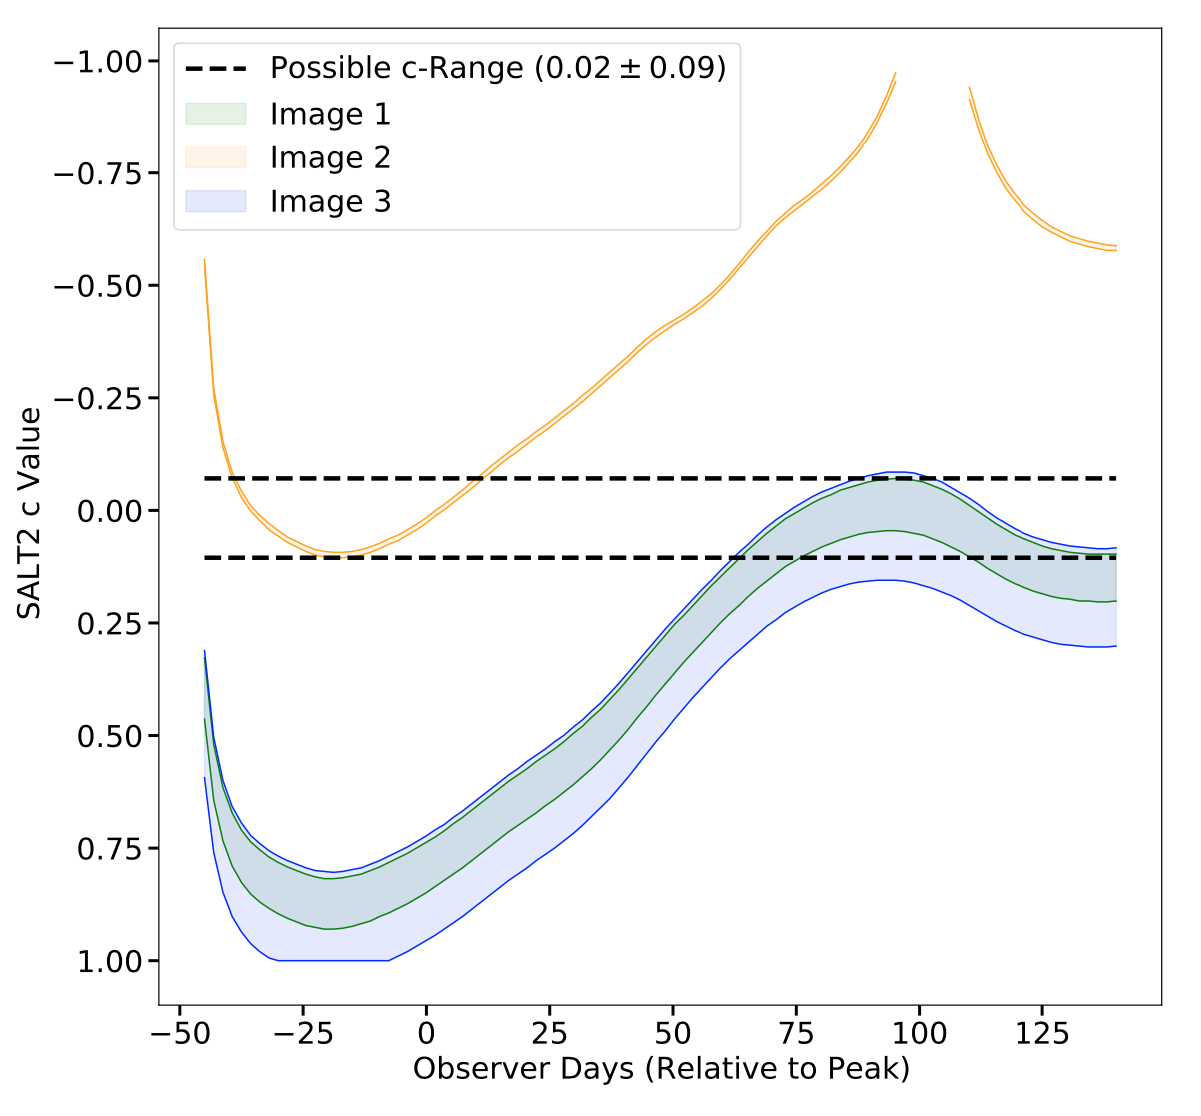
\includegraphics[width=0.7\textwidth]{Paper/ResponseToReferees/snrequiem_color_constraints.png}
    \caption{The SALT2-color vs. Observer-frame Phase. The serindipitous positioning of the three SN images is highly effective for a joint constraint on SALT2 c.  This figure is for illustrative purposes only---meaning that we did not use this construction for placing constraints on the SN color or phase. }
    \label{fig:salt2c_vs_phase}
\end{figure}
\clearpage
\else
\fi

\two{The waters turn even muddier when looking at Fig. S6 showing the bimodal nature of the fits, rendering the quoted SN ages, and especially their uncertainties, hard to defend. E.g., the central value for the quoted ages of Images 1 and 2 seem to be sitting at a local minimum of their probability distribution. If I have misunderstood this, others may as well. Thus, a clarification is needed.}{

Yes, the referee is highlighting here an issue of presentation that we wrestled with.  We were torn about how to present the interpretation of these bimodal distributions.  We expect that future observations of the final appearance of the SN will provide better constraints on the intrinsic light curve shape, which would collapse those distributions to one mode or the other.  Therefore, the expected final  precision of each parameter would be accurately represented by picking a single peak from the distribution. However, there is no good way to collapse the degeneracy in advance.    We opted for a concise presentation of the uncertainty, though it was somewhat muddy.

Happily, this problem has resolved itself.  After correcting the book-keeping error on the photometry described above (using the wrong flux column), we have re-run the time delay fitting with SNTD and find that the posterior distributions are significantly  less bimodal.   \hlt{Figures 9 and 11} now show these corrected  distributions.  As you can see from our combined constraints in the updated Figure 11 on \hlt{p.36},
the 50th percentile is no longer at a local minimum for any parameter. We have opted therefore to still use the 16th and 84th percentiles to report the uncertainties in the text. }


\two{Issue \#3: The big picture, precision\\\\
Figure 3 in the paper, and the text that goes with it, argues for the competitiveness of events like AT2016tbd (assuming 4 more are found) as precision tools for cosmology. This is a bit of a stretch. First of all, the time scales involved, decades(!), hardly argues in favor of this being a very competitive probe. It is not even clear what instruments will be around to measure the light curve of fourth de-magnified image of AT2016tbd, and get a spectrum to finally settle on the classification. Furthermore, it is clearly not so that a 1\% uncertainty on time-delay (which is small enough for the lensing model considered) require AT216tbd like systems, with two decades between multiple images. The median uncertainty on the light curve peak MJD of the Pantheon compilation of SNIa used in cosmology is under 0.3 days, indicating that systems with time-delays of $>$50 days are already at that level of accuracy, if a SN cosmology type of light curve sampling is performed.}{

The referee's skepticism is understandable, but we feel that this essentially boils down to a cost/benefit analysis.  SN Requiem represents a class of objects that is not currently getting much consideration in cosmological projections (indeed, we have been guilty of overlooking cluster-lensed SNe ourselves—Pierel et al. 2021).   In this section of the paper we are not arguing that pursuit of other cosmological probes should be abandoned, but rather that cluster-lensed SNe should be included in the conversation.   For example, suppose that a future Roman Space Telescope GO program is approved, with fields that include strong-lensing clusters (someone will surely write that proposal).  This paper should help make the case for that GO program to use a cadenced observing strategy to enable detection of more AT 2016tbd-like events.    

The source-to-lens redshift ratio is another aspect of AT 2016tbd-like events that makes them interesting as additions to the cosmological toolkit.  As shown in Fig. 3, the contours in cosmological parameter space are highly complementary with other lensed SN time delays, due primarily to the unusually high redshift ratio of a typical cluster lens relative to galaxy-scale lenses.   

Regarding the future observations of AT 2016tbd, we have complete confidence that there will be suitable observatories available for follow-up.  Even if there is no space telescope for high-resolution imaging to capture the light curve, we can count on the availability of ground-based AO imaging with NIR detectors in the 2030's and beyond.  Furthermore, the ground-based ELTs will be excellent for spectroscopic classification.  High S/N spectroscopy can even be used to measure lensed SN time delays (Johansson et al. 2021, Bayer et al. 2021).  

Regarding the precision of other lensed SN time delay measurements:  unfortunately the precision on the time of peak measurement from the Pantheon sample is not representative of what we can expect from lensed SNe.   For light curves from ground-based observatories like LSST, most lensed SNe will have blended PSFs from multiple overlapping SN images.  One must also consider microlensing effects that perturb a lensed SN light curve (and are more problematic for galaxy-lensed SNe than cluster-lensed events like AT 2016tbd).    All analyses to date that have incorporated some of these complications have found that there is a floor of about +- 3 days, even for very high-quality light curves such as those expected from the Roman Space Telescope (Huber+ 2019, Pierel+ 2021).    As an absolute floor, one could look to the analysis of Goldstein et al. 2018, which found that microlensing of galaxy-lensed LSST SNe leads to a minimum uncertainty of 1\% to 4\% on the time delay, though this analysis assumed 45 observations with an HST-like system delivering  ``infinite signal-to-noise, with a uniform temporal spacing, spanning the light curve."

\noindent\url{https://ui.adsabs.harvard.edu/abs/2021MNRAS.502..510J}\\
\url{https://ui.adsabs.harvard.edu/abs/2021arXiv210106229B}\\
\url{https://ui.adsabs.harvard.edu/abs/2019A\%26A...631A.161H}\\
\url{https://ui.adsabs.harvard.edu/abs/2018ApJ...855...22G}
}


\one{It should be noted that images 1 and 3 are minima which are less susceptible to high deviations owing to microlensing compared to image 2 which is a saddle. }{

We have added this point in the \hlt{blue text on page 29, lines 425-426.}\\

Under our assumption that this SN is of Type Ia, we constrain the age of the SN at image 2 to be at or before peak brightness. This age is well within the projected ``achromatic phase'' of microlensing ($\sim$3 rest frame weeks after explosion), so our use of the SALT2 color curve to constrain the time delay for image 2 will be minimally impacted by microlensing.   If the magnitude of image 2 was significantly biased by microlensing, then we would expect the light-curve-based time delay estimate to be significantly different from the color-curve-based time delay estimate.  The fact that these two methods agree does reinforce the hypothesis that there are no extreme microlensing impacts on the SN images. }


\section{Lens Modeling}

\one{Table 1: What do the errors on magnification correspond to in Table 1?}
{ The magnifications listed in Table 1 are derived from the lens modeling.   As with the components of the mass model, the magnification uncertainties are derived from the MCMC models by sampling their posterior probability distribution (see the Lens Modeling section of the supplementary materials).   For a detailed analysis of magnification uncertainties in the LENSTOOL modeling framework, we would refer the reader to the original LENSTOOL paper (Jullo et al. 2007).\\ \url{https://iopscience.iop.org/article/10.1088/1367-2630/9/12/447}} 

\one{Why are the absolute errors so small for SN images 1 and 4?}{
\textit{Note: after adjusting the labeling of the SN images to match Newman et al. 2018, the previous image 1 is now image 3.  So this comment refers to the lens model predictions for the magnifications of SN images 3 and 4, reported in Table 1 as 3.9$\pm$0.5 and 0.4$\pm$0.2, respectively.}\\
These represent the uncertainty from the final lens model, E, and give the formal 16-84\% confidence interval of the distribution of magnifications derived from the MCMC sampling done by LENSTOOL.  They are therefore statistical uncertainties only, and do not reflect possible systematics related to choices in the setup of the lens model.  Newman et al. 2018 explored systematic uncertainties for the magnifications of this MRG0138 cluster by constructing variants of their LENSTOOL model.  Those authors found systematic uncertainties of 30\% to 43\%.    We have similarly explored variations in the LENSTOOL modeling (models A through E, as described in the Lens Modeling section in the Methods addendum).  The range of magnifications across these five model variants can is reflected in the magnitude uncertainties shown in Figure 2 
(and again in \hlt{Figure 6} in the Methods section).   When classifying the transient, we have used the full range of magnification uncertainties across all 5 lens model variants—so we are in fact using an estimate of the systematic uncertainties for the SN analysis.   
These last points were not clear in the originally submitted text, so we have added text to clarify \hlt{(green text, page 25, lines 339-341).}}


\one{Please add predictions for image 5 in the table. }{

This refers to \hlt{Table 1, now on page 12}
We have updated Table 1 to show the lens model E magnification (basically $<0.01$ in all models) and time delay predictions for SN image 5.}


\one{Do the authors understand why the time delays are so poorly constrained?}{
The lens model has poor constraints for the time delays primarily because of the limited number of physical constraints in the immediate vicinity of the transient source.   For MACS J0138 we have three multiply-imaged systems to use.  For comparison, the lens models of the cluster MACS J1149 that were used to make time delay predictions for SN Refsdal began with 10 multiply-imaged galaxies, and were updated to include 30 individual knots within the face-on spiral that was the SN Refsdal host galaxy (Treu et al. 2016).   We can not hope that MACS J0138 will ever yield quite that richness of lens model constraints, but it could certainly be improved in coming years.   This is addressed in our new note in the supplemental note ``Future observations" \hlt{(p.41-42).}
}

\one{Couldn't the relative magnifications of the SN1-3 be used to get more accurate predictions for the time delay? In fact, one may even want to go with the assumption that the transient is truly a SN1a and make use of the absolute magnifications to better constrain the lens model and see how the time delay predictions are affected.}{
It would indeed be interesting to incorporate magnifications as constraints, though this would be at the cost of a fully blinded analysis, which is methodologically valuable.    An example of using the magnification of lens-magnified Type Ia SN to test lens models was presented in Rodney et al. 2015 (\url{https://ui.adsabs.harvard.edu/abs/2015ApJ...811...70R/abstract}).   With a full light curve of the lensed SN from the fourth image (c.\,2037), one could derive a measurement of the peak apparent magnitude in the B band, $m_B$.  Then one could use the collection of non-magnified Type Ia SNe at similar redshifts to provide a prediction for what is the ``expected" peak magnitude, thus delivering a measure of the lensing magnification for AT 2016tbd that is largely free of cosmological assumptions (see Rodney+ 2015 for details).   This, however, will be limited in the near term by the dearth of well-measured Type Ia SNe at $z\sim2$.   By 2037 we can expect that the $z\sim2$ SNIa sample will be substantially expanded by, for example, the Roman space telescope survey, so this kind of analysis should in fact be possible.   The new ``Future Observations" supplementary note discusses this  possibility \hlt{(pages 41-42)}}

\one{Cluster lenses are better for cosmology because they produce longer time delays but they also have more complex mass distribution and tend to have relatively massive structures in the line-of-sight which can affect the observables (e.g. see the spread in the SN Refsdal predictions of magnification vs time delay in Kelly et al. 2016). These caveats need to be mentioned and that different challenges exist at both galaxy and cluster-scales. }{

We absolutely agree that cluster lens modeling is a very different beast than galaxy-scale lens modeling, and both have distinct challenges.   We have updated the text to more clearly acknowledge this, and also took the opportunity to highlight the value of cluster lens modeling as a means for testing systematics. \hlt{ (blue text, page 7, lines 142-146)}
}


\one{ The radial magnification of image 4 and the position of the image 5 are not included as data constraints which is probably going to affect the constraints on the density profile and as a result magnification along with the time delays. Why are these constraints not taken into account?}{

The Lenstool code is not structured to allow the use of observed fluxes as a constraint when using image plane optimization.   It can only be done when using source plane optimization.   We find the image plane optimization is more robust here compared to source plane optimization because it deals better with actual positional uncertainties.   

We recognize that additional lens modeling of this cluster could use alternate approaches that may be informative, and may improve on our model predictions.  We hope that this work will encourage such efforts.  }


\one{  Newman et al. have used pixel data as constraints from images 1-3 and attempted sophisticated modelling of the lens. The model predicted images 4 and 5 can be compared with the data in their paper. How does the preferred model E compare with that of Newman et al. e.g. predicted magnifications of H1-H3 from their rough Sersic models? Does the preferred model predict the location of Image 5 correctly ? }{

This is a very good suggestion to provide a more explicit comparison to the Newman et al. (hereafter N18) model predictions.   We have added a new Supplementary Note \hlt{(p.39-40)} that compares our lens model E against the N18 lens modeling methodology and magnification predictions.
This is referenced in the lens modeling discussion on \hlt{p.21 (lines 278-281)}.

The new \hlt{Supplementary Table 1 on p.39} shows that our magnification predictions are fully consistent with the N18 values, when comparing the flux ratios averaged over each galaxy image profile.    Our model E does yield systematically lower magnification predictions compared to the N18 model.   This is consistent with our own estimate of lens modeling systematics (our lens model variants A-D also yield higher magnifications than model E).    We note that slightly higher magnifications would in fact result in a more “normal” SNIa absolute luminosity. 
}

\one{Table S4: The velocity dispersions for the BCG and other components in the table look unrealistically small. My assumption is that PIE parameters are not too different from the SIE model. How could this produce such a large image separation in the lensed images?  Also, the rcore for the DM component is too big compared to the rcut. These parameters look very strange. One cannot just rely on Bayesian evidence.}{
\textit{(Note: this is now \hlt{Table 5 on p.19})}\\

Thank you for noticing this.  We made a mistake when converting that table into Latex.  We mixed up the ordering of columns between $r_{cut}$, $r_{core}$, and $\sigma$.  This resolves the issues the referee pointed out, and it is now corrected in the resubmitted manuscript.}

\one{ Isn't there any measurement of the stellar velocity dispersion of the BCG which could constrain sigma in the model instead of keeping it free ?}{
At the referee's suggestion, we have measured the velocity dispersion of the BCG from our MUSE data, finding it to be 390$\pm$10 km s$^{-1}$. We now report this measurement in the Methods section, \hlt{blue text, page 15, lines 211-214}.

We explored the effect of including this in model E, but we did not develop a complete new model with this additional constraint.  At this point, such a model would not be blind, and therefore would require a separate discussion in the paper to describe its impact on the SN classification and time delay.  This would be difficult to do within the limits of a Nature Astronomy letter.  

Though we prefer to restrict ourselves to the blind model E in this paper, future work on this cluster could and should incorporate the measured BCG velocity dispersion. With a preliminary extension of model E we have explored what the impact will be, and find it will likely be within the range of our current systematic uncertainty estimates.  See the new Supplementary Note on Future Lens Modeling \hlt{(blue text, p.40-41)}
}

\one{Since only the positions of the lensed images are used as constraints, the mass model possibly doesn't have many degrees of freedom. }{
This is a reasonable point, and certainly argues for the value of future lens modeling work on this cluster. The Newman et al. lens modeling did include pixel-level constraints, and we are encouraged that our model predictions for the magnifications are very consistent with that work (see the new Lens Model Comparison section in the Methods). We feel that the mass model is sufficiently well-constrained for the purposes of this paper (classification and preliminary predictions). To actually use this SN for cosmology, a revised lens model will be warranted (and there is plenty of time to build that model!). We anticipate future lens models will leverage all of the pixel-level data from Newman et al. 2018, along with new data that we are publishing in this paper: positions and magnitudes of the SN and the measured velocity dispersion of the BCG. To aid in comparison of those future lens models with our predictions, we are publishing the pixel-by-pixel source model and residuals from our preferred lens model (model E).}


\one{Many of the model E parameters are fixed a priori which are probably coming from the previous models (i.e. A-D). If yes, then the best fit parameters of model E are not independent of the previous models and one cannot use the Bayesian evidence to decide which of these models are preferred. How were the model E parameters fixed a priori? }{
To fix the model E parameters {\it a priori}, we did not take values from the previous model fit and hold them constant.  Rather, we used the result of the previous model as a guide to choose {\it which} parameters should be fixed in order to get a useful improvement with the next model.  We then used observed information to set the actual a priori constraints.   This is admittedly a subtle point, and does somewhat cloud the interpretation of the Bayesian evidence analysis.  As we've revised this document, we find that the Bayesian evidence discussion is not essential to the main conclusions of the paper, and have simply removed it. 
}

\three{Page 6: The authors quote a 5\% uncertainty from lens modeling, with the potential to improve to 2\% precision with improved lensing constraints. Is this just from statistical uncertainty? What about potential systematics? In the lensed quasar community, there has been quite a lot of recent debate about systematics arising from mass profiles (see e.g., Blum+2020, Kochanek 2020a,b, Birrer+2020), and I would suspect that clusters, being more complex, would have similar issues. Also, what about potential line-of-sight effects (e.g., external convergence)}{

We agree that there is good reason to be cautious when using cluster lens models for predicting time delays or magnifications at specific locations.  Most public lens models on well-studied clusters were not designed for time delay cosmography.   Because of this, the scatter in predictions from such lens models should not necessarily be taken as an indication of the true systematic uncertainty from a model that is well constrained and designed for the task.  As an example, the most effective models designed for predicting the time delays of SN Refsdal are already able to deliver uncertainties of $<$7\% in a fully blind analysis. 

It’s true that there are known parameter degeneracies in lens modeling that could contribute a systematic error term on the order of 10\%.  However, work such as Birrer et al. 2016,2020 and Birrer \& Treu 2020 propose methods to significantly reduce these impacts by way of high-quality velocity dispersion measurements and a hierarchical Bayesian modeling methodology.   Line-of-sight effects may be mitigated by 3D and multi-plane lens modeling (e.g., McCully et al. 2014, Chirivi et al. 2018, Raney et al. 2020, Buckley-Greer et al. 2020).  

We believe that further progress on these methods alone may be sufficient to limit the total lens modeling uncertainty to $\sim$5\%.  Finally, under the assumption of the SN being of Type Ia we expect high-quality spectroscopy and photometry for the final image to provide additional constraints to guard against lens modeling systematics.  

Even if our prognosis for more precise and robust cluster lens models proves overly optimistic, we would argue that cluster-lensed SN are still valuable in time delay cosmography.  The systematic biases of cluster lens models will always be very different from those of galaxy scale lens modeling.   The vast majority of time delay cosmography constraints will likely come from quasars lensed by galaxy-scale lenses.   As we have attempted to show in Figure 3,  just a handful of cluster-lensed SNe with precision comparable to SN Requiem will be valuable for validating the full time delay sample.
\noindent\url{https://ui.adsabs.harvard.edu/abs/2014MNRAS.443.3631M}\\
\url{https://ui.adsabs.harvard.edu/abs/2018A\%26A...614A...8C}\\
\url{https://ui.adsabs.harvard.edu/abs/2020MNRAS.492..503R}\\
\url{https://ui.adsabs.harvard.edu/abs/2020MNRAS.498.3241B}\\
}


\three{Lens Modeling section: How many individual cluster galaxies are included in the lens model? It might be useful to include a figure similar to Figure 1, indicating the location of the mass components (pointing out the four galaxies that are individually optimized), as well as the multiply-imaged features that constrain the model.}{
There are 32 individual cluster galaxies included in the lens model. Including the BCG, three perturbers, and the main cluster potential, there are 37 components in total for lens model E.  We have added a sentence in the text and a figure to show them \hlt{(p 17 lines 236-237 and Fig 4)}
}

\three{Lens Modeling section: Could the authors include a figure showing the ``reproduced" arc morphology with model E and the two Sersic sources? It's difficult to evaluate this statement without seeing the reconstructed image.}{
We have produced this figure and included it in the Methods section \hlt{(Fig 5 on p 20, referenced on page 19, line 272)}
}


\section{Other Miscellaneous Comments}

\one{Abstract says ``Hubble constant''. Add ``LeMaitre'' too.}{Done (but now in the second paragraph due to rewording of the ``abstract'' to fit Nat.Astro. style)}

\one{Add Quimby et al. 2014 reference as it claimed to have a lensed SN Ia.}{Done}

\one{In Fig. 1 or in a new figure, identify the measured image positions of source at $z=0.766$ (3.1-3.4), H1-4 and SN1-4 along with the predictions of model E.}{Fig 1 now includes the locations of the multiply-imaged galaxy system 3.1-3.4}

\three{Figure 1: It would be helpful if this figure indicated the locations of the multiply-imaged features used to constrain the lens model (the ones listed in Table S3). The text states that the ``central light peak'' of the SN host galaxy is used - presumably this is the brightest pixel at the center of each galaxy image? The images of the background galaxy at z=0.766 should be indicated as well (was the central light peak also used)?}{
Fig 1 now includes the locations of the multiply-imaged galaxy system 3.1-3.4.

The ``central light peak''  refers to the centroid position of each galaxy image, determined from the source extraction algorithm applied on the HST F105W imaging.  We have clarified this in the main text \hlt{(maroon text, page 5, line 84)}.}


\one{Fig. 3 Caption: Dashed lines are too close together and almost appear as solid lines unless seen at a highly zoomed version. White marker is transparent which appears colored due to multiple overlapping colored contours. Making it black would help.}{We have updated the figure as suggested.}

\two{ Can the authors please enlighten the readers as to what the expected rate of discoveries may be?}{

We have added a few paragraphs discussing expected rates into the new Supplementary Note section on  Future Discoveries \hlt{(green text, page 42)}.   We note, however, that the published work on this is quite limited, and we hope this paper will encourage more  effort in this direction.    The rate estimates we have cited are based on a small number of lensing clusters, and for various methodological reasons should be seen as lower limits on the expected rates.   Extrapolating these (crudely) over the next 10-15 years, we anticipate at least 10 detections each from the LSST and Roman surveys.    A more accurate estimation would include a much more complete census of lensing clusters, along with lens models to predict magnifications and time delays, and measurements of star formation and stellar mass in lensed galaxies to predict the SN explosion rate.   This is a substantial undertaking, which we would prefer to leave for future work. }

\one{Fig S3 and S5 Captions: Typo in ``image 1 (upper right)''. It will be upper left.}{
Corrected.  (These are now \hlt{Figure 8 on p 33 and Figure 10 on p. 35)}}


\one{Table S3: ID 3.1-3.4 are not identified in the image of the lens system. Could the authors point these out in Fig. 1 or show in supplementary figures?}{
Done.  Figure 1 now includes labels for images 3.1-3.4}

\one{Image order is strange. They don't seem to be ordered by apparent magnitude, time delay or magnification. Couldn't the authors keep the same numbering order as Newman et al.? It creates unnecessary confusion otherwise.}{
We have corrected this by swapping the labels for SN images 1 and 3 throughout—in figures, tables and text.   Perhaps the long delay in responding to the referee's report will mean that you've conveniently forgotten which image was which, and the swap will not be confusing. }

\one{Page 4 says 2037 +/- 1.5 whereas everywhere else the error is given as 2 yrs.}{Corrected.}

\three{Table S7: The quantities in the table should have uncertainties associated with them.}{
Corrected.  \hlt{(this is now Table 6 on p.19)}}

\two{To summarize: I am charmed by the beautiful discovery. However, I find that the current manuscript makes unnecessary claims on the cosmological implications. I don’t think these are necessary to publish a discovery paper on this rare phenomenon.}{

We appreciate your enthusiasm for the discovery itself.   Our long delay in this response notwithstanding, we are also still charmed by it.    We hope that our response and the improvements in the text spurred by your comments will persuade you that the cosmological discussion is worthy of inclusion.} 


\end{document}